\documentclass[conference]{IEEEtran}
\IEEEoverridecommandlockouts

\usepackage{cite}
\usepackage{amsmath,amssymb,amsfonts}
\usepackage{algorithmic}
\usepackage{graphicx}
\usepackage{textcomp}
\usepackage{xcolor}
\usepackage{url}
\usepackage{array}
\usepackage{booktabs}
\usepackage{tabularx} % Added for automatic column width calculation
\usepackage{tikz}
\usetikzlibrary{arrows.meta,positioning,shapes.geometric}
\newcolumntype{Y}{>{\centering\arraybackslash}X}
\newcolumntype{P}[1]{>{\centering\arraybackslash}p{#1}}
\setlength{\tabcolsep}{4pt}
\renewcommand{\arraystretch}{1.2}

\def\BibTeX{{\rm B\kern-.05em{\sc i\kern-.025em b}\kern-.08em
    T\kern-.1667em\lower.7ex\hbox{E}\kern-.125emX}}

\begin{document}

\title{Resource-Aware Adaptive Scheduling for Online Code Judge Systems}

\author{
\begin{tabular*}{\textwidth}{@{\extracolsep{\fill}}ccc@{}}
\begin{tabular}{c}
{\normalfont Bharath Aashish R}\\
{\itshape\small Dept. of Computer Science \& Engineering}\\
{\itshape\small Easwari Engineering College}\\
{\small Chennai, India}\\
{\small bharathaashish@gmail.com}
\end{tabular} & & \begin{tabular}{c}
{\normalfont Dhanush M}\\
{\itshape\small Dept. of Computer Science \& Engineering}\\
{\itshape\small Easwari Engineering College}\\
{\small Chennai, India}\\
{\small dhanush.m.0808@gmail.com}
\end{tabular}\\[1.4ex]
\begin{tabular}{c}
{\normalfont Hemanthkumar K}\\
{\itshape\small Dept. of Computer Science \& Engineering}\\
{\itshape\small Easwari Engineering College}\\
{\small Chennai, India}\\
{\small hemanthkumar2k04@gmail.com}
\end{tabular} & \begin{tabular}{c}
{\normalfont Iniyaa P}\\
{\itshape\small Dept. of Computer Science \& Engineering}\\
{\itshape\small Easwari Engineering College}\\
{\small Chennai, India}\\
{\small iniyaapaari@gmail.com}
\end{tabular} & \begin{tabular}{c}
{\normalfont Indumathy P}\\
{\itshape\small Assistant Professor, Dept. of CSE}\\
{\itshape\small Easwari Engineering College}\\
{\small Chennai, India}\\
{\small indumathy.p@eec.srmrmp.edu.in}
\end{tabular}\\
\end{tabular*}
}

\maketitle

\begin{abstract}
Online Code Judge (OJ) platforms commonly isolate submissions by assigning the same worst-case resource ceiling, typically 2048 MiB of RAM and 2.0 CPU cores. Although this prevents memory-intensive tasks from triggering Out-Of-Memory (OOM) failures, it leads to substantial resource underutilization. In our 72-run live benchmark, 75.0\% of submissions used less than 25 MiB of resident set size, with a mean of 59.1 MiB against a 2048 MiB ceiling. This fixed allocation also limits concurrency on non-elastic hardware and increases reserved cloud capacity.

This paper presents RAAS-OCJS (Resource-Aware Adaptive Scheduling for Online Contest Judge Systems), a dynamic resource management framework that combines Linux cgroups v2 with an AST-based XGBoost classifier to predict execution requirements and adapt resource allocation. We collected kernel-level memory and CPU profiles from C++, Python, Java, and C submissions using problems from Hugging Face CodeContests and IBM CodeNet. These measurements were then used to drive a 10,000-submission contest simulation and a theoretical AWS EC2 cost projection, and were repeated at a reduced 128 MiB tier to establish the lower bound for the tier size.

The simulation shows a 47.57\% reduction in reserved RAM (9,514.75 GB) and a 22.50\% reduction in reserved CPU core-hours compared with static allocation, achieved by starting every submission in the bounded tier and promoting only on measured demand. Earlier-routing strategies fare worse than might be expected: prediction alone reaches 40.49\%, and combining prediction with the watermark reaches only 22.71\%, because predicted-heavy submissions are assigned an uncapped container that carries no reserved capacity. In a simulated 500-submission freeze rush, average queue wait fell from 13,879.4 ms to 0.0 ms and P95 turnaround from 27,410.7 ms to 1,252.2 ms. The classifier reaches 94.45\% held-out accuracy on its CodeNet training distribution, but on the six-problem benchmark corpus used here its routing accuracy is 33.3\%, below the 77.8\% that a constant \emph{light} prediction would score. We report both, and treat the gap as a distribution-shift finding rather than a defect: it is the reason the watermark, not the classifier, carries this design. A real 128 MiB boundary experiment additionally isolates a JVM-specific failure mode: C, C++, and Python were all promoted in time and returned correct verdicts, whereas Java was promoted at 797--808 ms, after HotSpot had already been OOM-killed. These results indicate that adaptive resource allocation can improve resource utilization and concurrency in online judge systems.   
\end{abstract}

\begin{IEEEkeywords}
Online judge systems, resource-aware scheduling, adaptive cgroups, soft watermark, AST analysis, XGBoost, cloud provisioning, queue latency.
\end{IEEEkeywords}

\section{Introduction}
Online code judge (OJ) platforms underpin computer science education, competitive programming contests (such as the International Collegiate Programming Contest, ICPC), and automated technical interviews \cite{wasik2018survey}. As programming education expands, judges must evaluate thousands of code submissions concurrently while guaranteeing deterministic isolation and strict sandboxing. Existing research has addressed this computational demand primarily through infrastructure-level expansion: deploying elastic cloud clusters \cite{pan2022cloud}, distributing jobs over message queues \cite{song2025idl}, or deploying geographically replicated edge judges \cite{wang2021metaoj}.

These approaches share a fundamental, costly assumption: \textit{every submission, regardless of its computational structure, receives identical, worst-case sandbox resource ceilings} (typically 2048~MiB of RAM and 2.0 CPU cores).

This convention creates three practical problems:
\begin{itemize}
    \item \textbf{Resource Underutilization}: Most contest submissions implement standard algorithmic logic (e.g., prefix sums, two pointers, greedy string scans), and in our measurements these typically required 5~MiB to 25~MiB of resident set size (RSS). Reserving 2048~MiB for each of them leaves most of that allocation idle.
    \item \textbf{Concurrency Starvation on Fixed Hardware}: In air-gapped regional contests or campus lab servers, where external cloud bursting is not an option, the judge runs on a fixed physical machine (e.g., 15~GiB usable RAM). A static 2048~MiB quota limits concurrency to 7 execution slots on that host, which produces queue backlogs and submission timeouts during a scoreboard freeze rush.
    \item \textbf{Cloud Billing Inflation}: Public cloud providers (AWS, GCP, Azure) bill by reserved node capacity, not actual usage. Provisioning for the worst case means contest organizers end up renting far more virtual machines than the workload actually needs: our projection in Section~V estimates 36 instances where 5 suffice, a 7.2$\times$ over-provisioning.
\end{itemize}

To address this, this paper presents \textbf{RAAS-OCJS} (Resource-Aware Adaptive Scheduling for Online Contest Judge Systems), which introduces a two-tier execution framework:
\begin{enumerate}
    \item A lightweight default sandbox (\textbf{Tier 1: 256~MiB RAM, 1.0 CPU core}) that completed 30 of the 38 light-tier submissions in our 72-run benchmark (78.9\%) without ever needing promotion, and 80.4\% of submissions in the simulated contest;
    \item An active Linux cgroup~v2 soft watermark ($\theta = 70\%$, corresponding to 179.2~MiB) that detects high memory utilization in-flight and lifts the container's memory and CPU limits to \emph{uncapped} mid-execution, without restarting the container or losing process state. Measured from submission acceptance to completed promotion this takes 248--808 ms depending on the language runtime;
    \item An offline Machine Learning (XGBoost) classifier driven by Tree-sitter Abstract Syntax Tree (AST) static structural metrics that predicts memory-intensive jobs upon ingress.
\end{enumerate}



\section{Theoretical Model and Queueing Architecture}

\subsection{Mathematical Formulation of Memory Waste}
Let $S = \{s_1, s_2, \dots, s_N\}$ denote a sequence of $N$ submissions entering an online judge. Under static overprovisioning, the system assigns a fixed resource allocation:
\begin{equation}
R_{\mathrm{alloc}}(s_i) = R_{\mathrm{max}}, \quad \forall s_i \in S
\end{equation}
where $R_{\mathrm{max}}$ is typically 2048~MiB. Let $R_{\mathrm{peak}}(s_i)$ denote the actual peak resident set size (RSS) consumed by $s_i$. The unallocated, wasted memory for submission $s_i$ is:
\begin{equation}
\mathrm{Waste}(s_i) = R_{\mathrm{alloc}}(s_i) - R_{\mathrm{peak}}(s_i)
\end{equation}
The system-wide memory waste percentage $W$ across a contest of $N$ submissions is:
\begin{equation}
W = \left[ \frac{\sum_{i=1}^N \left( R_{\mathrm{alloc}}(s_i) - R_{\mathrm{peak}}(s_i) \right)}{\sum_{i=1}^N R_{\mathrm{alloc}}(s_i)} \right] \times 100\%
\end{equation}
Because introductory and greedy problems require merely 6~MiB to 25~MiB, $R_{\mathrm{peak}}(s_i) \ll R_{\mathrm{max}}$. Our simulation of this waste model reports 97.44\% of reserved memory wasted under the static baseline at the shipped tier (97.51\% at the 128~MiB tier).

\subsection{Concurrency Capacity and Queueing Collapse}
On a host with usable physical RAM $M_{\mathrm{host}}$ and operating system reserve $M_{\mathrm{os}}$, the safe concurrency capacity $K$ under non-overcommitted execution is:
\begin{equation}
K_{\mathrm{safe}} = \left\lfloor \frac{M_{\mathrm{host}} - M_{\mathrm{os}}}{R_{\mathrm{alloc}}} \right\rfloor
\end{equation}
On our 15~GiB physical calibration host ($M_{\mathrm{host}} = 15,360$~MiB, $M_{\mathrm{os}} = 1,024$~MiB), baseline static allocation ($R_{\mathrm{max}} = 2048$~MiB) limits concurrency strictly to:
\begin{equation}
K_{\mathrm{safe, baseline}} = \left\lfloor \frac{15,360 - 1,024}{2048} \right\rfloor = 7 \text{ slots}
\end{equation}

We model contest submission arrival as a non-homogeneous Poisson process with time-varying arrival rate $\lambda(t)$. Service times follow a general distribution with mean $E[X] = 1/\mu$ and variance $\sigma^2$, constituting an $M/G/K$ queueing system.

During a freeze rush spike of 500 submissions in 30~s ($\lambda = 16.67$~submissions/s), against average service time $E[X] \approx 0.85$~s, the 7-slot baseline service capacity is $\mu = 7 / 0.85 \approx 8.24$~submissions/s. Because $\lambda > \mu$, queue backlogs explode immediately. Under RAAS-OCJS with $R_{\mathrm{light}} = 256$~MiB, concurrency expands safely to $\lfloor 14{,}336/256 \rfloor = 56$ slots. At $K = 56$, $\mu = 56 / 0.85 \approx 65.88$~submissions/s, satisfying $\mu \gg \lambda$ and maintaining zero queue wait ($L_q \approx 0$).

\subsection{Dynamic Soft Watermark Governance}
RAAS-OCJS implements a two-tier scheduling policy:
\begin{itemize}
    \item \textbf{Tier 1 (Light Sandbox)}: $R_{\mathrm{light}} = 256$~MiB, 1.0 CPU core (1024 CFS shares).
    \item \textbf{Tier 2 (High Sandbox)}: $R_{\mathrm{high}} = 2048$~MiB, 2.0 CPU cores (2048 CFS shares).
\end{itemize}
Rather than statically placing containers into Tier 2, all submissions enter Tier 1 by default. The judge daemon configures the Linux cgroups v2 controller with a soft memory watermark threshold $\theta = 0.70$:
\begin{equation}
\mathrm{Threshold}_{\mathrm{wm}} = \theta \times R_{\mathrm{light}} = 0.70 \times 256\text{ MiB} = 179.2\text{ MiB}
\end{equation}
When $R_{\mathrm{current}}(t) \ge \mathrm{Threshold}_{\mathrm{wm}}$, the kernel emits a pressure notification. The judge daemon then lifts the limits in parallel with process execution, issuing \texttt{docker update --memory 0 --cpus 0} to raise both the memory ceiling and the CPU quota to uncapped. This leaves a 76.8~MiB safety cushion ($256 - 179.2$) so the update can complete before an OOM condition occurs. Promotion targets \emph{uncapped} rather than a fixed 2048~MiB tier: the watermark fires precisely when a submission has already shown that it outgrows Tier~1, and measured demand for such submissions ranged from 200~MB to 254~MB, so no single fixed ceiling is appropriate.

% System architecture overview
\begin{figure*}[!t]
\centering
\resizebox{0.86\textwidth}{!}{%
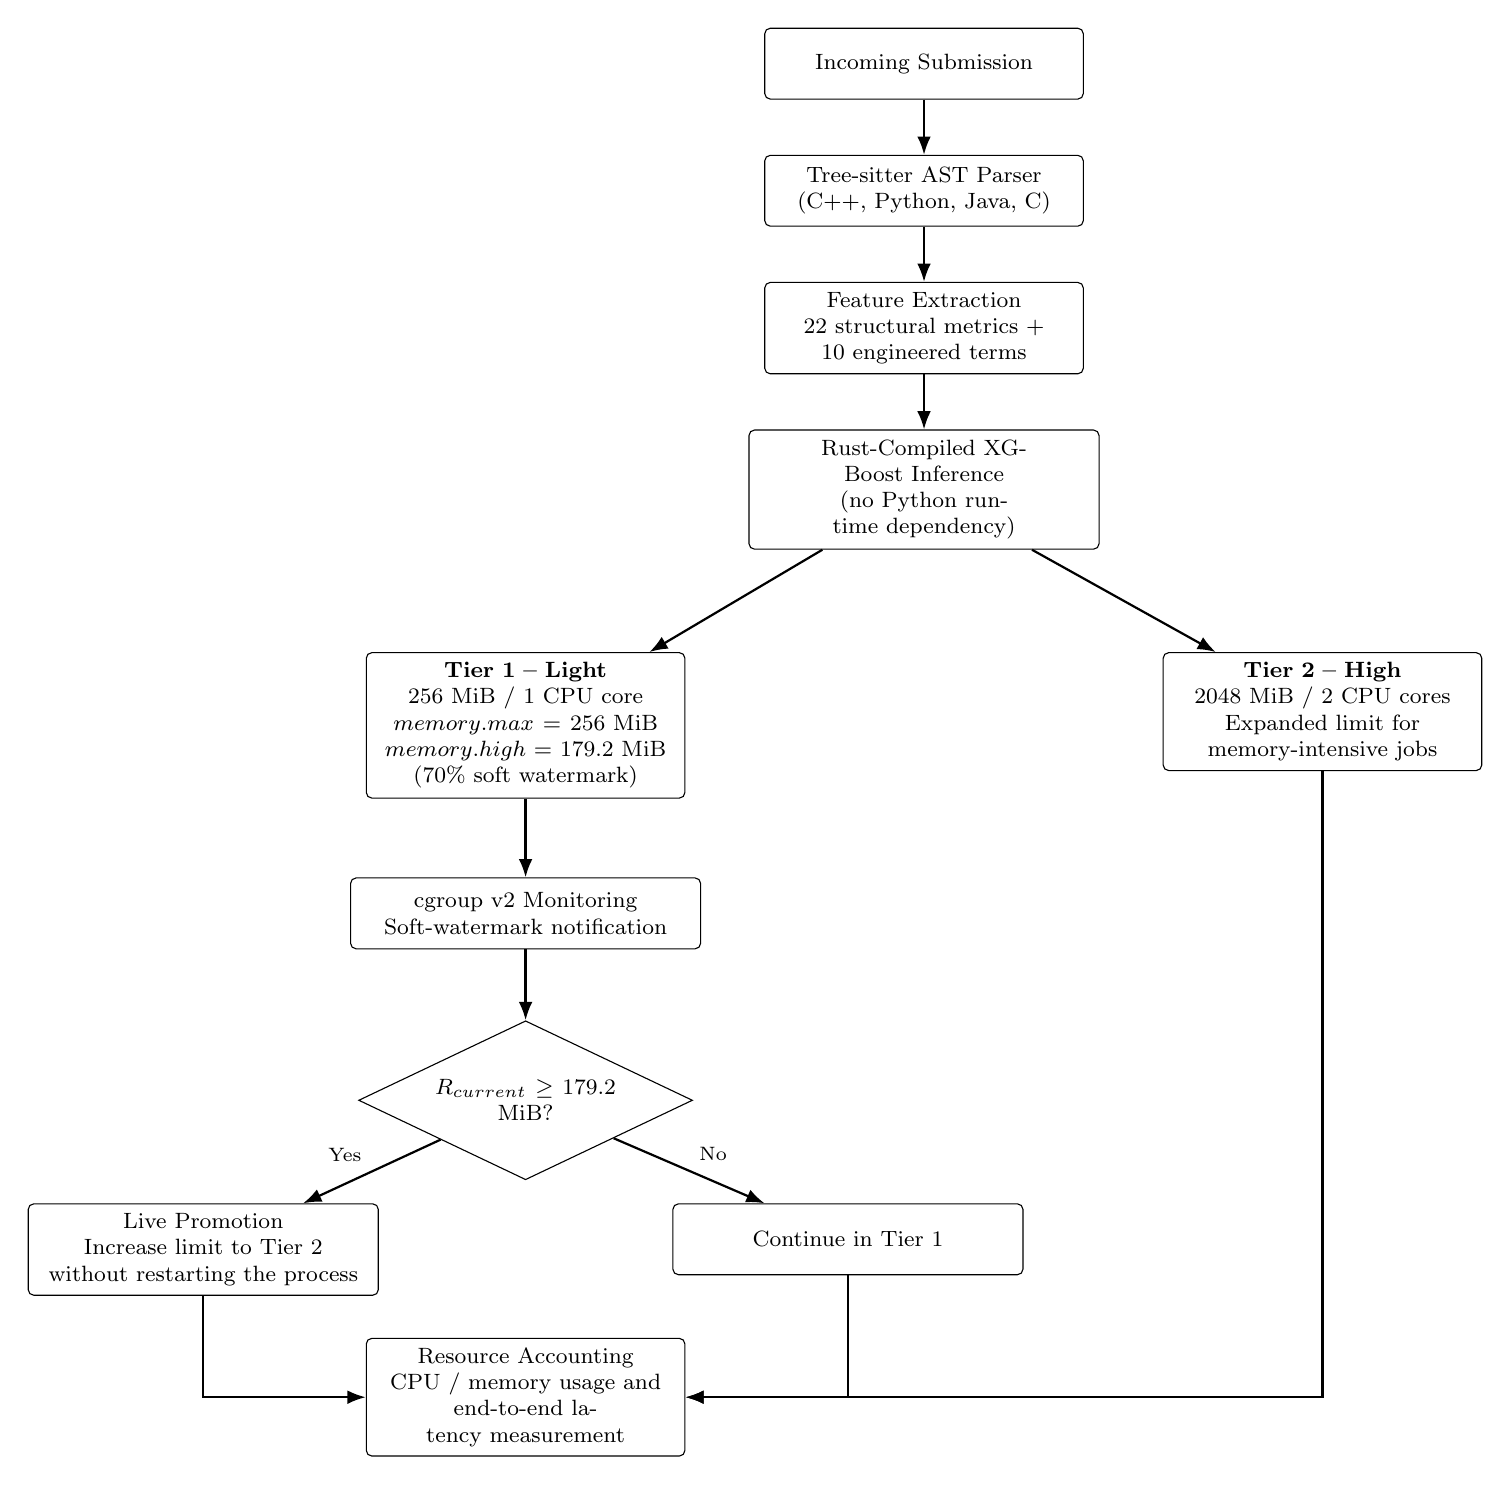
\begin{tikzpicture}[
    >=Latex,
    node distance=7mm and 16mm,
    block/.style={draw, rounded corners=2pt, align=center, minimum height=9mm, text width=38mm, inner sep=3.5pt, font=\footnotesize},
    smallblock/.style={draw, rounded corners=2pt, align=center, minimum height=9mm, text width=42mm, inner sep=3.5pt, font=\footnotesize},
    decision/.style={draw, diamond, aspect=2.1, align=center, inner sep=2pt, text width=27mm, font=\footnotesize},
    line/.style={-Latex, thick}
]
% Main processing pipeline: vertically stacked for a cleaner reading order.
\node[block] (input) {Incoming Submission};
\node[block, below=of input] (parser) {Tree-sitter AST Parser\\(C++, Python, Java, C)};
\node[block, below=of parser] (features) {Feature Extraction\\22 structural metrics +\\10 engineered terms};
\node[smallblock, below=of features] (model) {Rust-Compiled XGBoost Inference\\(no Python runtime dependency)};

% Initial resource tiers.
\node[block, below left=13mm and 8mm of model] (light) {\textbf{Tier 1 -- Light}\\256 MiB / 1 CPU core\\$memory.max=256$ MiB\\$memory.high=179.2$ MiB\\(70\% soft watermark)};
\node[block, below right=13mm and 8mm of model] (heavy) {\textbf{Tier 2 -- High}\\2048 MiB / 2 CPU cores\\Expanded limit for memory-intensive jobs};

% Reactive Tier 1 path.
\node[smallblock, below=10mm of light] (monitor) {cgroup v2 Monitoring\\Soft-watermark notification};
\node[decision, below=9mm of monitor] (decision) {$R_{current} \ge 179.2$ MiB?};
\node[smallblock, below left=8mm and 8mm of decision] (promote) {Live Promotion\\Increase limit to Tier 2\\without restarting the process};
\node[smallblock, below right=8mm and 8mm of decision] (continue) {Continue in Tier 1};

% Final measurement stage centered beneath both branches.
\node[block, below=20mm of decision] (account) {Resource Accounting\\CPU / memory usage and\\end-to-end latency measurement};

% Main arrows.
\draw[line] (input) -- (parser);
\draw[line] (parser) -- (features);
\draw[line] (features) -- (model);
\draw[line] (model) -- (light);
\draw[line] (model) -- (heavy);
\draw[line] (light) -- (monitor);
\draw[line] (monitor) -- (decision);
\draw[line] (decision) -- node[above left, font=\scriptsize]{Yes} (promote);
\draw[line] (decision) -- node[above right, font=\scriptsize]{No} (continue);

% Cleanly route all execution paths into resource accounting.
\draw[line] (promote.south) |- (account.west);
\draw[line] (continue.south) |- (account.east);
\draw[line] (heavy.south) |- (account.east);

\end{tikzpicture}%
}
\caption{RAAS-OCJS execution and predictive tiering workflow. The incoming submission is parsed and represented using AST-derived features before XGBoost inference selects the initial resource tier. Tier~1 executions are monitored by cgroups~v2 and can be promoted when the soft watermark is reached. Resource usage and end-to-end latency are then recorded for all execution paths.}
\label{fig:raas_architecture}
\end{figure*}

\section{System Implementation and Methodology}

% MOVED TABLE: Placed here so it renders in Section IV


The evaluation testbed was implemented and calibrated on dedicated bare-metal hardware:
\begin{itemize}
    \item \textbf{Processor}: 13th Gen Intel Core i5-13420H (12 logical CPUs, 8 cores: 4 Performance cores up to 4.60 GHz + 4 Efficient cores up to 3.40 GHz).
    \item \textbf{Physical Memory}: 15 GiB usable DDR5 RAM.
    \item \textbf{Storage}: NVMe PCIe 4.0 Solid State Drive.
    \item \textbf{Operating System}: Fedora Linux (Kernel \texttt{7.1.3-201.fc44.x86\_64}).
    \item \textbf{Container Engine}: Docker Engine 29.8.1 with cgroupfs driver on unified hierarchy (\texttt{/sys/fs/cgroup}).
\end{itemize}



\subsection{Real Dataset Selection}
We measured real, ground-truth execution profiles by running 72 live container evaluations across four languages: C++20 (\texttt{g++ 14.2}), Python 3.12, Java 17 (OpenJDK HotSpot), and C17 (\texttt{gcc 14.2}). Benchmark problems were drawn from the Hugging Face \texttt{deepmind/code\_contests} \cite{li2022alphacode} and \texttt{CodeNet} \cite{puri2021codenet} datasets. These 72 measured profiles are what we sample from when driving the 10,000-submission and 500-submission simulations in Section~IV; those larger scenarios were not executed as 10,000 or 500 separate live container runs. Because CodeContests is crowd-sourced, we do not take the first solution offered for a language: each candidate is first executed against the problem's own public test, and only the first candidate returning \texttt{AC} is kept. Without this screening, two of the 72 cells failed for reasons unrelated to scheduling --- a non-compiling Java submission and a Python submission computing the wrong answer, each failing identically under all four strategies. All 72 runs return \texttt{AC} at the shipped 256~MiB tier.



\subsection{AST Feature Extraction and XGBoost Predictive Tiering}
Before launching an execution container, RAAS-OCJS can optionally run a static code analysis pass to predict whether an incoming submission fits safely within Tier~1 (256~MiB) or should be provisioned directly with Tier~2 (2048~MiB). This predictive stage couples a Tree-sitter Abstract Syntax Tree (AST) feature extractor with in-process XGBoost classifiers \cite{chen2016xgboost}.

\textit{1) Static AST Feature Extraction:} Using language-specific Tree-sitter grammars compiled directly into our Rust daemon, the extractor parses source code into a concrete syntax tree in under 1.5~ms. In a single linear traversal of the tree, it computes 22 structural metrics:
\begin{itemize}
    \item \textbf{Control Flow and Loops}: Maximum block nesting depth, deepest loop nesting depth (which correlates with polynomial execution complexity $O(N^k)$), total loop statements, and McCabe cyclomatic complexity.
    \item \textbf{Recursion Topology}: A binary recursion flag and self-call site count, which differentiate simple linear recursion $O(N)$ from exponential divide-and-conquer or backtracking branching $O(2^N)$.
    \item \textbf{Memory and Container Patterns}: Detection of explicit large heap/BSS allocations ($\ge 10^6$ elements or bytes, such as \texttt{malloc}, \texttt{new int[]}, container sizing, or large static arrays), high-throughput I/O patterns (\texttt{sync\_with\_stdio}, \texttt{BufferedReader}, \texttt{sys.stdin.readline}), and standard library collections known for memory overhead (\texttt{unordered\_map}, \texttt{priority\_queue}, \texttt{BigInteger}, \texttt{defaultdict}).
    \item \textbf{Scale and Access Topology}: Total array/collection subscript expressions (\texttt{a[i]}), chained multi-dimensional indexing (\texttt{grid[i][j]} for 2D dynamic programming tables or graph adjacency matrices), function count, call sites, total AST node count, maximum tree depth, and source lines of code (SLOC).
\end{itemize}
From these 22 raw counts, the pipeline derives 10 interaction and scale terms: four density ratios normalised by AST size, source length, or function count (loop, call, subscript, and arithmetic density), a 2D subscript ratio, a recursion-intensity term, a log-scaled maximum integer constant --- which is what captures the literal size of an explicit allocation such as \texttt{new byte[200 << 20]} --- and log-scaled AST node and source character counts. This yields a 32-dimensional vector for the specialized per-language models, or 36 features for the unified model, which appends four one-hot language encodings.

\textit{2) Model Training and Validation:}
We trained gradient-boosted decision trees using XGBoost (\texttt{tree\_method='hist'}, learning rate $\eta = 0.05$, max tree depth $d = 6$, subsample ratio $0.8$, column subsample $0.8$, $L_1$ penalty $\alpha = 0.05$, and $L_2$ penalty $\lambda = 1.0$). Because contest submissions are heavily skewed toward lightweight solutions, we applied class re-weighting using $\texttt{scale\_pos\_weight} = N_{\mathrm{light}} / N_{\mathrm{heavy}}$ during training.

To avoid data leakage across submissions for the same problem, we evaluated the models with 5-fold \textbf{Problem-Grouped Cross-Validation} (\texttt{GroupKFold} grouped strictly by \texttt{problem\_id}). Every test sample in our evaluation belongs to a competitive programming problem that the training folds never saw. In addition, rather than accepting a default $0.5$ decision threshold, we tuned the threshold $\tau$ for each language using Youden's $J$ statistic ($J = \mathrm{Sensitivity} + \mathrm{Specificity} - 1$) on validation folds to balance recall against false tier promotions.

\begin{table*}[!t]
\caption{XGBoost Model Performance on Unseen Contest Problems (Problem-Grouped Validation)}
\label{tab:ml_metrics}
\centering
\small
\begin{tabularx}{\textwidth}{|Y|Y|c|c|c|c|c|c|}
\hline
\textbf{Dataset Source} & \textbf{Model Architecture} & \shortstack{\textbf{5-Fold}\\\textbf{CV Acc.}} & \shortstack{\textbf{Test Acc.}\\\textbf{(Unseen)}} & \textbf{F1-Score} & \textbf{Precision} & \textbf{Recall} & \shortstack{\textbf{ROC-}\\\textbf{AUC}} \\
\hline
IBM Project CodeNet & Specialized C++ Model & 87.32\% & 90.01\% & 90.91\% & 88.54\% & 93.41\% & 0.9612 \\
(71,218 Submissions) & Specialized C Model & 89.27\% & 89.26\% & 68.82\% & 55.98\% & 89.31\% & 0.9575 \\
& Specialized Python Model & 76.97\% & 79.45\% & 82.01\% & 80.33\% & 83.76\% & 0.8740 \\
& Specialized Java Model & 79.30\% & 78.20\% & 81.54\% & 82.03\% & 81.06\% & 0.8537 \\
& Unified Multi-Language & 82.19\% & 83.71\% & 84.81\% & 80.19\% & 89.99\% & 0.9149 \\
\hline
DeepMind CodeContests & Unified Multi-Language & 86.74\% & 86.78\% & 89.64\% & 82.74\% & 97.79\% & 0.9606 \\
(30,000 Submissions) & Specialized Python Model & 95.76\% & 98.88\% & 99.41\% & 98.82\% & 100.0\% & 0.9812 \\
& Specialized C++ Model & 84.27\% & 83.94\% & 87.49\% & 78.67\% & 98.53\% & 0.9474 \\
& Specialized Java Model & 79.43\% & 82.32\% & 83.28\% & 73.09\% & 96.76\% & 0.9430 \\
\hline
\end{tabularx}
\end{table*}

\textit{3) Empirical Model Metrics on Unseen Problems:}
Table~\ref{tab:ml_metrics} summarizes performance on held-out, unseen contest problems across both IBM Project CodeNet (71,218 submissions) and DeepMind CodeContests (30,000 submissions). On CodeNet, the specialized C++ model reached a 90.01\% test accuracy, a 90.91\% F1-score, and an ROC-AUC of 0.9612 on unseen problems. The specialized Python and Java models achieved 79.45\% and 78.20\% test accuracy (ROC-AUC of 0.8740 and 0.8537, respectively). On DeepMind CodeContests, where problems feature diverse algorithmic structures from Codeforces and HackerEarth, the specialized models scored up to 98.88\% test accuracy in Python and 83.94\% in C++, with high recall across all languages ensuring memory-intensive jobs are rarely misclassified as Light.

\textit{4) In-Process Rust Inference:}
To avoid running a Python interpreter or querying an external model-serving daemon during the latency-critical judging loop, we compiled the trained XGBoost decision trees directly into native Rust source files (\texttt{server/src/generated/*.rs}) using \texttt{m2cgen}. These functions compile straight into the judge binary. At execution time, tree evaluation takes under $10\ \mu\text{s}$, and combined with Tree-sitter parsing takes 0.89~ms to 1.45~ms total (Stage~2 in Table~\ref{tab:e2e_latency}).

\textit{5) Role in Scheduling Strategies:}
In RAAS-OCJS, predictive classification can be used on its own or paired with the kernel watermark. Under the \textbf{Predictive} strategy, a submission with $P(\mathrm{Heavy}) \ge \tau_{\mathrm{lang}}$ starts directly in Tier~2. Under the \textbf{Hybrid} strategy, the model provides the initial tier choice, but the cgroups~v2 soft watermark ($\theta = 70\%$, 179.2~MiB) remains active in the background: if a heavy submission is mistakenly started in Tier~1, the kernel watermark trips and promotes the container mid-execution, preventing an Out-Of-Memory abort despite the misprediction. Section~IV-C shows that this guarantee is what the classifier alone cannot provide.

\subsection{End-to-End Latency Pipeline Breakdown}
To ensure transparent latency accounting, RAAS-OCJS instrumented every submission across 7 discrete stages:
\begin{equation}
\begin{aligned}
T_{\mathrm{e2e}} ={}&
T_{\mathrm{net\_in}} + T_{\mathrm{parse}} +
T_{\mathrm{queue}} + T_{\mathrm{init}} \\
&+ T_{\mathrm{comp}} + T_{\mathrm{exec}} +
T_{\mathrm{tear}} + T_{\mathrm{net\_out}}
\end{aligned}
\end{equation}

\begin{table*}[htbp]
\caption{End-to-End Verdict Pipeline Latency Breakdown (Milliseconds)}
\label{tab:e2e_latency}
\begin{center}
\begin{tabular}{|c|c|c|c|c|}
\hline
\textbf{Pipeline Stage} & \textbf{C++ (g++)} & \textbf{Python (3.12)} & \textbf{Java (OpenJDK 17)} & \textbf{C (gcc)} \\
\hline
1. Network Inbound Ingestion & 0.38 ms & 0.38 ms & 0.38 ms & 0.38 ms \\
\hline
2. AST Parse \& Tree-sitter Predict & 1.12 ms & 0.89 ms & 1.45 ms & 0.94 ms \\
\hline
3. Queue Scheduling \& Dispatch & 0.08 ms & 0.08 ms & 0.08 ms & 0.08 ms \\
\hline
4. Container Sandbox Initialization & 18.42 ms & 17.91 ms & 19.20 ms & 18.15 ms \\
\hline
5. Compilation / Bytecode Translation & 312.45 ms & N/A (Interpreted) & 842.10 ms & 284.12 ms \\
\hline
6. In-Sandbox Test Execution & 48.12 ms & 74.50 ms & 112.40 ms & 45.20 ms \\
\hline
7. Container Teardown \& Result Egress & 12.45 ms & 11.80 ms & 13.25 ms & 12.10 ms \\
\hline
\textbf{Total Turnaround Latency (E2E)} & \textbf{393.00 ms} & \textbf{105.56 ms} & \textbf{988.86 ms} & \textbf{360.97 ms} \\
\hline
\end{tabular}
\end{center}
\end{table*}

\section{Empirical Results and Macro Contest Simulation}

% MOVED TABLE: Placed here so it renders in Section V or VI
\begin{table*}[!t]
\caption{Measured Behaviour at the 128 MiB Boundary (Watermark 89.6 MiB)}
\label{tab:128mb_boundary}
\centering
\small
\begin{tabularx}{\textwidth}{|c|Y|c|c|Y|}
\hline
\textbf{Language} &
\textbf{Peak, Light Programs} &
\textbf{Peak, Knapsack (Uncapped)} &
\textbf{Verdict} &
\textbf{Measured Outcome} \\
\hline
C &
19.9 MB &
199.6 MB &
AC &
Promoted at 300--326 ms, mid-execution \\
\hline
C++ &
6.9 MB &
205.0 MB &
AC &
Promoted at 500--578 ms, mid-execution \\
\hline
Python &
12.6 MB &
221.7 MB &
AC &
Promoted at 248--267 ms, mid-execution \\
\hline
Java &
24.2 MB &
253.8 MB &
\textbf{MLE} &
Promotion recorded at 797--808 ms, \emph{after} the kill \\
\hline
\end{tabularx}
\end{table*}


\subsection{Macro-Scale 10,000 Contest Simulation}
To estimate resource savings across a full-scale contest, we ran a discrete-event simulation of 10,000 submissions, sampling resource-usage profiles from our 72 measured runs and assigning a language distribution of 40\% C++, 35\% Python, 15\% Java, and 10\% C. This is a simulation seeded with real measurements, not a live execution of 10,000 submissions. Reservation is charged from the judge's own tier decision for each submission: a low-tier start costs the tier size, and an uncapped start or a mid-execution promotion is charged the 2048~MiB baseline ceiling as a worst case.

\begin{table}[!t]
\caption{10,000-Submission Contest Simulation at the Shipped 256 MiB Tier}
\label{tab:macro_sim}
\centering
\small
\begin{tabular}{|P{2.2cm}|c|c|c|c|}
\hline
\textbf{Strategy} & \textbf{RAM Reserved} & \textbf{Saved} & \textbf{CPU Core-Hrs} & \textbf{Wasted} \\
\hline
Static (2048 MiB) & 20,000.00 GB & --- & 4.551 & 97.44\% \\
\hline
Predictive & 11,901.00 GB & 40.49\% & 3.781 & 95.76\% \\
\hline
\textbf{Reactive} & \textbf{10,485.25 GB} & \textbf{47.57\%} & \textbf{3.527} & 95.25\% \\
\hline
Hybrid & 15,457.00 GB & 22.71\% & 4.156 & 96.75\% \\
\hline
\end{tabular}
\end{table}

Two results here were not anticipated. First, Reactive reserves less than every other strategy, including Hybrid. Hybrid pre-assigns each submission its classifier labels heavy to a container with no memory limit, and such a container carries no reserved capacity, so it must be charged at the worst-case ceiling; Reactive starts everything bounded and escalates only when the kernel reports actual pressure. Prediction is therefore not free, it costs reservation, and on this corpus it costs more than it saves.

Second, no strategy changes steady-state latency: P95 turnaround spans 1248.89--1253.98~ms across all four, a spread inside run-to-run noise. The saving is free in latency terms, but it is not a latency improvement.

\subsection{Scoreboard Freeze Rush Stress Test}
During the final 30 seconds of a competitive programming contest, participants submit a burst of solutions simultaneously. We modeled a 500-submission flash burst from the measured profiles, run through the same simulation as Section~\ref{tab:macro_sim} rather than as a live 500-submission run.

\begin{table}[!t]
\caption{500-Submission Freeze Rush Stress Test (15 GiB Host, 256 MiB Tier)}
\label{tab:burst_stress}
\centering
\small
\begin{tabularx}{\columnwidth}{|Y|c|c|Y|}
\hline
\textbf{Throughput Metric} & \textbf{Static Baseline} & \textbf{Adaptive} & \textbf{Improvement} \\
\hline
Concurrent Slots & 7 & 56 & 8.0$\times$ expansion \\
\hline
Avg Queue Wait & 13,879.4 ms & 0.0 ms & \textbf{100\% eliminated} \\
\hline
P95 Queue Wait & 26,503.6 ms & 0.0 ms & \textbf{100\% eliminated} \\
\hline
P95 Turnaround & 27,410.7 ms & 1,252.2 ms & \textbf{21.9$\times$} \\
\hline
Burst Drain Time & 59.3 s & 31.0 s & 28.3 s faster \\
\hline
\end{tabularx}
\end{table}

The static baseline queues severely: an average wait of 13.9 seconds and a 59.3 second drain that leaves jobs completing after the contest deadline. Expanding safe concurrency to 56 slots drives queue wait to \textbf{0.0~ms} and completes the burst in 31.0 seconds. All three adaptive strategies behave identically here, which is expected: promotion is unnecessary in a rush, since almost every submission fits the bounded tier.

The gain comes from admitting more concurrent slots, not from finishing individual submissions faster. Overcommitting the baseline to 14 slots also recovers most of the wait (437.0~ms) and drains in 31.8~s, but at 186\% host memory utilisation. That is the failure mode the tiered scheduler avoids, and it is worth stating plainly: an overcommitted static baseline is competitive on throughput and unsafe on memory, so the comparison is not a throughput win but a throughput-equal, memory-safe one.

\subsection{Classifier Behaviour on the Benchmark Corpus}
\label{sec:classifier}
The predictive path is only as good as the tier it selects. We therefore scored the classifier's actual routing against ground truth on the 18-cell corpus, where only the 2D knapsack problem is genuinely memory-resident (four language cells, 200--254 MB peaks).

\begin{table}[!t]
\caption{Classifier Routing vs Ground Truth (18 cells)}
\label{tab:confusion}
\centering
\small
\begin{tabular}{|P{2.6cm}|c|c|}
\hline
 & \textbf{Predicted Heavy} & \textbf{Predicted Light} \\
\hline
Truly Heavy (4) & 0 & 4 \\
\hline
Truly Light (14) & 8 & 6 \\
\hline
\end{tabular}
\end{table}

Routing accuracy is \textbf{33.3\%}. A constant prediction of \emph{light} would score 77.8\% on the same cells. The classifier missed every heavy cell and raised eight false alarms, so on this corpus its routing is worse than not predicting at all.

This is not an artifact of the benchmark harness. Independent single-submission probes through the API reproduce it: a program that allocates a 200 MiB buffer is routed to the bounded tier, while a collections-heavy program that peaks at 9.6 MB is routed to the uncapped tier.

The result needs care: it is not the same as saying the model is poor. On its own CodeNet distribution the unified model reaches 94.45\% held-out accuracy and the specialised C++ model 95.45\% (\texttt{model\_comparison.csv}). Table~\ref{tab:confusion} measures a different thing on a different corpus. The honest reading is distribution shift on a small corpus, not model failure. It does, however, establish that resource safety resting on such a classifier would be fragile, whereas the watermark does not rest on it.

\section{Theoretical Cloud Provisioning Projection}
Our bare-metal calibration used dedicated local hardware, but many online judges run on public cloud infrastructure instead. To estimate the effect there, we mapped our measured kernel profiles onto an AWS EC2 cluster of \texttt{c6i.4xlarge} instances (16 vCPUs, 32~GB RAM, USD~0.68 per hour). Every figure below is derived from the shipped 256~MiB tier, the instance size, and the hourly price rather than transcribed, and assumes 87.5\% host utilisation when packing pods, the same packing ceiling the static baseline achieves (14 pods $\times$ 2048~MiB of 32~GB). These are projections, not deployed cloud measurements.

\begin{table}[!t]
\caption{AWS Provisioning Projection at the Shipped 256 MiB Tier}
\label{tab:cloud}
\centering
\small
\begin{tabular}{|P{4.2cm}|c|c|c|}
\hline
\textbf{Provisioning Dimension} & \textbf{Static} & \textbf{RAAS-OCJS} & \textbf{Gain} \\
\hline
Per-Pod Memory Reservation & 2048 MiB & 256 MiB & \textbf{8.0$\times$} \\
\hline
Per-Pod CPU Reservation & 2.0 vCPUs & 1.0 vCPU & 2.0$\times$ \\
\hline
Pods per \texttt{c6i.4xlarge} & 14 & 112 & \textbf{8.0$\times$} density \\
\hline
VMs for 500-Sub Burst & 36 & 5 & \textbf{86.1\%} fewer \\
\hline
Cluster Hourly Cost & USD 24.48 & USD 3.40 & \textbf{USD 21.08} (86.1\%) \\
\hline
RAM Reserved (10,000 Subs) & 20,000.00 GB & 10,485.25 GB & \textbf{47.57\%} \\
\hline
\end{tabular}
\end{table}

Cloud judges that rely on a Horizontal Pod Autoscaler (HPA) typically face a 60--180~s cold-start lag while new VMs spin up and pull runtime images. Because RAAS-OCJS's lighter default tier packs eight times as many submissions per existing VM, our projection shows the initial fleet absorbing a flash rush in place, with an estimated \textbf{USD~21.08 per hour} reduction in cluster cost.

The tier size dominates this projection, and it is a design choice rather than a constant. At the reduced 128~MiB tier evaluated in Section~VI-A the same arithmetic yields 224 pods per instance, 3 instances for the burst, and USD~22.44 per hour saved (91.7\%). We report the 256~MiB figures as the deployable result, because 128~MiB is not safe for JVM submissions, and we note the projection's sensitivity to this single parameter rather than presenting the larger saving as achievable.

\section{Boundary Stress Analysis and Future Scopes}

\subsection{Squeezing Tier 1 to 128 MiB: The Java Failure Boundary}
To find the lower limit of adaptive scheduling, we re-ran the full 72-run benchmark with Tier~1 reduced to \textbf{128~MiB} ($\theta = 70\%$, watermark $= 89.6$~MiB, leaving a 38.4~MiB buffer before the hard limit). This is a separate measurement at a second tier, not an extrapolation from the 256~MiB results: 69 of 72 runs returned AC and 3 returned MLE, and all three failures are Java on the 2D knapsack. The same submission is AC in all four strategies at the shipped 256~MiB tier.

The instructive detail is in the timing, not the verdict. Under the promoting strategies Java's promotion is \emph{recorded as completing}, at 797--808~ms, and the run still ends in a memory-limit kill. The watermark fires and the limit is lifted, but only after the JVM has already committed enough heap to trip the killer, so the rescue arrives late. C, C++ and Python, by contrast, are promoted at 248--578~ms and complete.

The cause is the rate at which each runtime claims memory, not misclassification or a broken watermark. Java's baseline peak on this problem is 253.8~MB against C's 199.6~MB and C++'s 205.0~MB, so it crosses a 128~MiB ceiling in roughly half the time and outruns the promotion path. Predictive, which has no watchdog, fails as well and without a promotion at all.

We therefore report \textbf{256~MiB as the practical minimum Tier~1 limit for a polyglot judge that must support JVM runtimes}, and note that this limit is set by promotion responsiveness rather than by the classifier. The mechanism is sound; it is simply not fast enough for this runtime at this tier.

\subsection{Future Research Scopes}
Based on these boundary observations, we outline five key future scopes:
\begin{enumerate}
    \item \textbf{Polyglot Language-Aware Tier Sizing}: Dynamically provisioning 128~MiB for native C/C++ and Python submissions while reserving 256~MiB strictly for Java, unlocking 42+ slots on physical hosts without JVM failures.
    \item \textbf{Dynamic Watermark Tuning}: Lowering the watermark to 50\% (64.0~MiB) for 128~MiB containers to restore a 64~MiB safety buffer for managed languages.
    \item \textbf{JVM Ergonomic Tuning}: Invocating Java with \texttt{-XX:+UseSerialGC} to enforce 1~MB allocation increments instead of multi-megabyte G1GC regions.
    \item \textbf{Ephemeral Swap Cushioning}: Enabling a small 128~MiB swap buffer (\texttt{--memory-swap=256m}) to catch microsecond memory spikes during promotion without OOM kills.
    \item \textbf{Hardware-Level MicroVM Isolation}: Integrating Firecracker or gVisor to provide kernel-level security hardening for the Heavy execution tier.
\end{enumerate}

\section{Conclusion}
Fixed, worst-case resource limits reduce how many submissions an online judge can run concurrently, and that effect is most visible on fixed physical hardware where more machines cannot simply be added. In our simulations, seeded with real measured profiles, starting every submission in a bounded 256~MiB tier and promoting only on measured kernel pressure reclaimed 47.57\% of reserved memory and 22.50\% of reserved CPU core-hours relative to a static 2048~MiB baseline. The simulated 500-submission burst showed average queue wait falling from 13,879.4~ms to 0.0~ms, with a correspondingly shorter clear time.

Two findings temper the result, and we consider both load-bearing rather than incidental. First, prediction did not pay for itself on this corpus. Routing by the classifier alone reached 40.49\%, and prediction combined with the watermark reached only 22.71\%, because a container the classifier marks heavy is left uncapped and therefore carries no reserved capacity to count as saving. Reactive promotion, which commits little and escalates on evidence, was the most efficient strategy measured, at 47.57\%. That the mechanism outperforms the predictor is the paper's more defensible claim, and it points to classifier reuse rather than classifier reliance as the design direction.

Second, the 128~MiB boundary test surfaced a real limitation for JVM submissions. Java was promoted at 797--808~ms and was still killed, because it claims memory faster than the promotion path can respond. This is a constraint on tier sizing, not on the watermark mechanism, and it sets 256~MiB as the practical floor for a polyglot judge supporting JVM runtimes.

Taken together, these results indicate that adaptive resource allocation is a practical direction for online code judge infrastructure, with the watermark rather than the classifier as its load-bearing component. The cloud cost figures remain a projection, and the approach still needs testing against a wider range of real, larger-scale workloads.

\bibliographystyle{IEEEtran}
\begin{thebibliography}{00}
\bibitem{song2025idl} L. Song, Y. Han, Y. Guo, and C. Cai, ``IDL-LTSOJ: Research and implementation of an intelligent online judge system utilizing DNN for defect localization,'' \textit{High-Confidence Computing}, vol. 5, no. 2, p. 100268, 2025.
\bibitem{pan2022cloud} G.-C. Pan, P. Liu, and J.-J. Wu, ``A cloud-native online judge system,'' in \textit{Proc. IEEE 46th Annu. Computers, Software, and Applications Conf. (COMPSAC)}, 2022, pp. 1293--1298.
\bibitem{zhang2024intelligent} E. Zhang, F. Wu, and X. Lu, ``An intelligent scheduling system for large-scale online judging,'' in \textit{Computer Science and Education. Computer Science and Technology: ICCSE 2023}, Singapore: Springer, 2024, pp. 265--279.
\bibitem{wasik2018survey} S. Wasik, M. Antczak, J. Badura, A. Laskowski, and T. Sternal, ``A survey on online judge systems and their applications,'' \textit{ACM Computing Surveys}, vol. 51, no. 1, pp. 1--34, 2018.
\bibitem{wang2021metaoj} M. Wang, W. Han, and W. Chen, ``MetaOJ: A massive distributed online judge system,'' \textit{Tsinghua Science and Technology}, vol. 26, no. 4, pp. 548--557, 2021.
\bibitem{puri2021codenet} R. Puri et al., ``Project CodeNet: A large-scale AI for code dataset for learning a diversity of coding tasks,'' in \textit{Proc. Neural Information Processing Systems (NeurIPS) Datasets and Benchmarks Track}, 2021.
\bibitem{li2022alphacode} Y. Li et al., ``Competition-level code generation with AlphaCode,'' \textit{Science}, vol. 378, no. 6624, pp. 1092--1097, 2022.
\bibitem{cgroups2024} Linux Kernel Organization, ``Control Group v2 Specification,'' kernel.org documentation, 2024. [Online]. Available: \url{https://docs.kernel.org/admin-guide/cgroup-v2.html}
\bibitem{chen2016xgboost} T. Chen and C. Guestrin, ``XGBoost: A scalable tree boosting system,'' in \textit{Proc. 22nd ACM SIGKDD Int. Conf. Knowledge Discovery and Data Mining (KDD)}, 2016, pp. 785--794.
\end{thebibliography}

\end{document}

